\chapter{Control Unit and Sign Extender}

\section{Control Unit}
Next, we will create the main control unit.  You will create a new module called control (in control.v) in 2\_decode.  The control module should use a portion of the instruction to determine the values of all control signals to be used in our processor.  These signals include:
\begin{enumerate}
\item reg2\_loc
\item uncondbranch
\item branch
\item mem\_read
\item mem\_to\_reg
\item alu\_op
\item mem\_write
\item alu\_src
\item reg\_write
\end{enumerate}

The supported instructions should include:
\begin{enumerate}
	\item ADD
	\item SUB
	\item AND
	\item ORR
	\item LDUR
	\item STUR
	\item CBZ
	\item B
\end{enumerate}

You will need to evaluate the incoming opcode and set the value of the control lines according to Figure~\ref{fig:control_value_table}.  Note that a value of X in a table entry indicates that it does not matter whether the value is 0 or 1.  You do not want to use X for these values, as this indicates 'undefined' to Verilog.  Instead, please use 0 in place of X.

The Verilog implementation between 'if/else' statements and 'case' statements differ.  'If/else' statements will create a series of nested muxes with two inputs each, whereas a case statement will produce one large mux with many inputs.  To maximize speed, we should use case statements. Note that all Verilog case statements must have a default case. But one of the challenges of this lab is dealing with opcodes of different sizes.  Thankfully, Verilog has 'casex', which will only evaluate binary digits that are not labeled X.  So for a CBZ instruction, you can fill in the last 3 digits with XXX and use 'casex'.  The 'casex' syntax will also be very helpful in the Sign Extender.  Also, please create macros in definitions.vh for the opcodes of each instruction and for the ALU Op values of each instruction type.  The values in the opcode macros can include X's when necessary so that they work appropriately with the casex.  For opcode macros, use the instruction type in all caps.  For instance, your macro for a load instruction should be LDUR.  For ALU Op macros,  use the following macro names:
\begin{enumerate}
	\item ALUOp\_RTYPE
	\item ALUOp\_DTYPE
	\item ALUOp\_B
	\item ALUOp\_CBZ
\end{enumerate} 

The default case should set all control signals to 0 to "turn off" the datapath in case of an invalid opcode.  The ALU Op should be R Type.

\begin{figure}
	\caption{Control Value Table}\label{fig:control_value_table}
	\begin{center}
		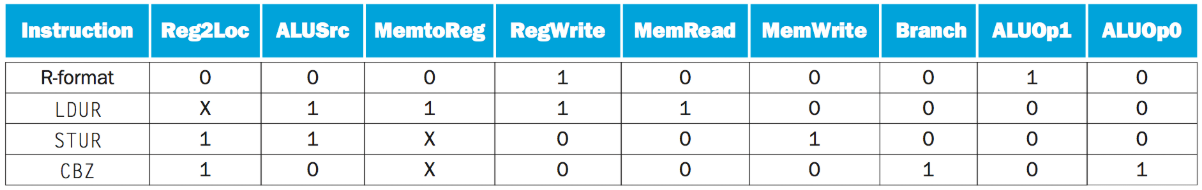
\includegraphics[width=4.75in]{../images/control_value_table.png}
	\end{center}
\end{figure} 

Note that you should not use a clk in this module.

\section{Control Unit Test}
The Control Unit is crucial to operation of your datapath, so it needs to be tested thoroughly.  Every supported instruction (listed above) should be tested with the Control Unit Test.  To facilitate testing, I have provided a testbench that includes all opcodes and an invalid opcode.  You just need to fill in the 'er' values.

\section{Sign Extender}
The final major component of the Decode stage is the Sign Extender.  The Sign Extender should use information in the instruction to create a 64-bit output value to use as an address or branch offset.  You need to extract the constant value from the instruction (this will be different for each instruction type), place that extracted value in the least significant bits of the sign\_extended\_output, then sign extend that value.  For positive values, the sign extender should fill extended bits with 0s.  For negative values, the sign extender should fill the extended bits with 1s.  The sign extender should support extending address values from the following instructions:
\begin{enumerate}
	\item LDUR
	\item STUR
	\item CBZ
	\item B
\end{enumerate}
For R-Type instructions that do not have a value to sign extend, please use the default case and set the value to 0.

Note that you should not use a clk in this module.

\section{Sign Extender Test}
The Sign Extender Test is provided for you with all 'er' values filled in.  However, half of the instructions are missing.  The comments indicate what the instructions should be, and you must fill in the missing instructions with the correct machine code.

\clearpage
\section{Your Assignment}

You are to:
\begin{enumerate}
\item Create a control module.
\item Update control\_test.sv with the correct 'er' values and verify that your control module works properly.
\item Create a Sign Extender module.
\item Update sign\_extender\_test.sv to fill in the missing instructions, then verify that your sign extender module works properly.
\item Produce a landscape mode PDF called Lab5\_lastname.pdf that includes (in this order):
\begin{enumerate}
	\item Your name and the lab number.
	\item A snip of the Simulation Results for the control module.  Please show opcodes in hex and everything else in binary.  
	\item A snip of the test results from the Tcl Console for the control module.  This snip should show the entire log from BEGIN TEST RESULTS to END TEST RESULTS.
	\item A snip of the Simulation Results for the sign\_extender module.  Please show instructions in hex and everything else in signed decimal.  
	\item A snip of the test results from the Tcl Console for the sign\_extender module.  This snip should show the entire log from BEGIN TEST RESULTS to END TEST RESULTS.	
\end{enumerate}
\item Upload Lab5\_lastname.pdf file to Canvas.
\item Zip up your ARM-Lab directory and submit it on Canvas as well.  I will run your code against my correct testbench to verify that your code and testbench work correctly.
\end{enumerate} 